% Compiler ce document 

% package de base
\documentclass[10pt,a4paper]{article}
\usepackage[utf8]{inputenc}
\usepackage{listings}

% langues
\usepackage[usenames,dvipsnames]{xcolor}
\usepackage[francais]{babel}
\usepackage[T1]{fontenc}
\usepackage{amsmath}
\usepackage{amsfonts}
\usepackage{amssymb}
\usepackage{graphicx}
\usepackage{tabularx}
\usepackage{colortbl}
\usepackage[hidelinks]{hyperref} % liens
\usepackage{fancyhdr} % En tetes / bas de page
\usepackage{helvet} % police helvetica
\usepackage[hidelinks]{hyperref}
\usepackage{xcolor} % Style pour affichage du C
\usepackage{courier} % police pour les listings

\usepackage{listingsutf8}

% Page de Garde -- Necessite d'installer le package titling, si probleme
% commenter la ligne suivante ainsi que les infos necessaires a la page
% de garde
\usepackage{pageGarde/HEIG_STY}

% commande pour faire des sections sans nombre 
% tout en la rajoutant dans la table des matières
\newcommand\sectionWithoutNumber[1]{\section*{#1} \addcontentsline{toc}{section}{\protect\numberline{}#1}}
\newcommand\subsectionWithoutNumber[1]{\subsection*{#1} \addcontentsline{toc}{subsection}{\protect\numberline{}#1}}
\newcommand\subsubsectionWithoutNumber[1]{\subsection*{#1} \addcontentsline{toc}{subsubsection}{\protect\numberline{}#1}}
% définition de nouvelles couleurs
\definecolor{lightblue}{rgb}{0.8,0.8,0.9}
\definecolor{grossblue}{rgb}{0,0,0.7}
%marge des pages
\setlength{\textwidth}{16cm}
\setlength{\textheight}{24cm}
\setlength{\oddsidemargin}{0cm}
\setlength{\voffset}{-1.5cm}
\setlength{\headheight}{15pt}

% set la police en arial
%% Sans-serif Arial-like fonts
\renewcommand{\rmdefault}{phv} 
\renewcommand{\sfdefault}{phv} 
\usepackage{tabularx}
\usepackage{graphicx}
\usepackage{eurosym}
\usepackage{xspace}
\newcommand{\projectname}[0]{LTANR\xspace} 

% configuration pour des listings
\lstset{ 
  showspaces=false,      
  showstringspaces=false, 
  showtabs=false,               
  tabsize=3,                     
  numbers=left
}

%enlève indentation en début de paragraphe
\setlength\parindent{0pt}

%style de l'en-tête de page
\pagestyle{fancy}

% style pour code en c
\lstdefinestyle{customc}{
  belowcaptionskip=1\baselineskip,
  breaklines=true,
  frame=L,
  xleftmargin=\parindent,
  language=C,
  showstringspaces=false,
  basicstyle=\scriptsize\ttfamily,
  keywordstyle=\bfseries\color{green!40!black},
  commentstyle=\itshape\color{purple!40!black},
  identifierstyle=\color{blue},
  stringstyle=\color{orange},
}

\lstdefinelanguage{VHDL}{
      morekeywords=[1]{
        library,use,all,entity,is,port,in,out,end,architecture,of,
        begin,and,or,Not,downto,ALL
      },
      morekeywords=[2]{
        STD_LOGIC_VECTOR,STD_LOGIC,IEEE,STD_LOGIC_1164,
        NUMERIC_STD,STD_LOGIC_ARITH,STD_LOGIC_UNSIGNED,std_logic_vector,
        std_logic
      },
      morecomment=[l]--
    }
    \usepackage[usenames,dvipsnames]{xcolor}
    \colorlet{keyword}{blue!100!black!80}
    \colorlet{STD}{Lavender}
    \colorlet{comment}{green!80!black!90}
    \lstdefinestyle{vhdl}{
      language     = VHDL,
      basicstyle   = \footnotesize \ttfamily,
      keywordstyle = [1]\color{keyword}\bfseries,
      keywordstyle = [2]\color{STD}\bfseries,
      commentstyle = \color{comment}
      breaklines=true,                % sets automatic line breaking
      tabsize=3                                % sets default tabsize to 2 spaces
    }

\lstset{escapechar=@,style=customc}
\lstset{inputencoding=utf8/latin1} %affiche les accents dans le listing

% Mise en forme de la page de titre
\author{João Miguel Domingues Pedrosa \\
Loïc Haas\\
Rick Wertenbroek}
\title{Decode Network Trace et Drum Challenge \\ Laboratoire 1}
\dest{Laboratoire 1}

% Informations necessaires a la page de garde
% Commenter si probleme de compilation
\acro{MCS}
\matter{Modern Concurent Systems}
\date{\today}

%en-tête
\lhead{Domingues, Haas \& Wertenbroek}
\chead{Laboratoire 1}
\rhead{\theAcro}

%pied-de-page
\lfoot{HEIG-VD}
\cfoot{\today}
\rfoot{\thepage}

\begin{document}
\maketitle
\newpage
\tableofcontents
\newpage

%Ici commence réelement l'écriture du rapport

\section{Drum challenge}

\subsection{Résumé du problème}

L'objectif de ce laboratoire est d'analyser un fichier sous forme binaire afin de pouvoir obtenir un affichage cohérent. Il n'y a pour seule aide le format de l'affichage désiré à nous d'étudier les fichiers binaires et de voir comment en extraire les informations.

\subsection{Décomposition du fichier binaire}

Les valeurs à décoder sont contenues dans un fichier possédant l'extension \texttt{.splice}. Il en a été fourni 5 avec leur affichages désirés respectifs.\\

Pour s'aider à trouver la manière dont les informations étaient encodées, nous avons utilisé le logiciel \texttt{hexinator} permettant l'affichage du contenu d'un fichier binaire en valeur hexadécimal ou ASCII.

\begin{figure}[ht]
	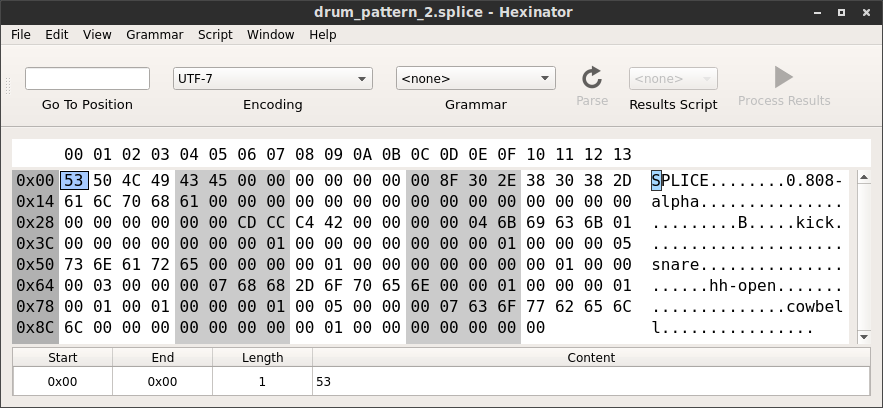
\includegraphics[scale=0.51]{images/hexa.png}
	\caption{Exemple de ce que nous sort Hexinator}
\end{figure}

Avec la comparaison des différents fichiers fournis et leur affichage désiré nous avons retiré les informations suivantes:
\begin{itemize}
    \item Header
    \begin{itemize}
		\item 6 octet: magic word (indique le type fichier)
		\item 8 octet: longueur en octets des informations restantes
		\item 32 octet: Nom de la version hardware (big-endian)
		\item 4 octet: tempo en float (little-endian)  
    \end{itemize}
    
    \item Tracks	
    \begin{itemize}
    	\item 1 octet: identifiant numérique
    	\item 4 octet: taille du nom de l'instrument (big-endian)
    	\item n octet: nom de l'instrument 
    	\item 4 * 4 octet: la mesure décomposée en 4 quarter de 4 battement
    \end{itemize}
\end{itemize}

À noter que les informations arrivent dans ce même ordre. La taille du header est constante pour chaque fichier. Par contre la taille des tracks change, parce qu'il peut y en avoir plusieurs dans un fichier et parce que le nom de l'instrument varie.

\newpage

\subsection{Parsing des informations}

\subsubsection{Header}
Afin de pouvoir parser le header, nous avons réalisé la fonction suivante:

\lstinputlisting[firstline=54, lastline=60,language=erlang]{sources/drum_sample.erl}

Nous commençons par regarder si le magic word est juste sinon on revoie un tuple contenant le type d'erreur ainsi que le binaire en brut. On récupère un payload de la taille définie par la valeur lue précédement. Il a été fait ainsi car il n'est possible d'avoir des octets en trop, cela n'est pas considéré comme une erreur. Ils doivent être ignorés d'où le dernier pattern matching. On peut voir ce cas dans le 5ème fichier pattern:

\begin{figure}[ht]
	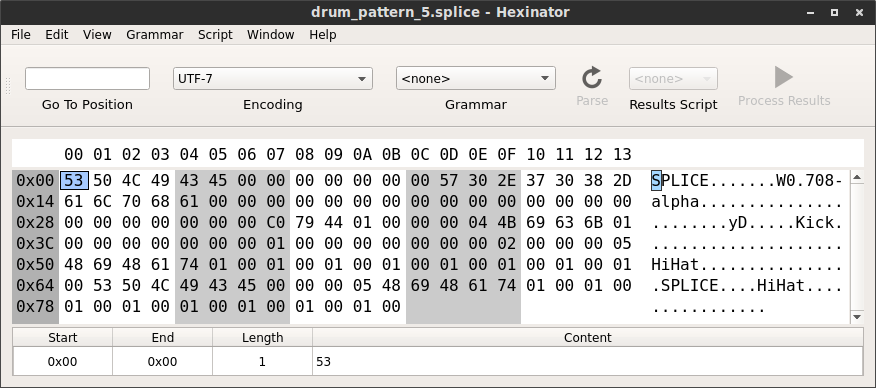
\includegraphics[scale=0.51]{images/hexa_fail.png}
	\caption{Ici, le payload fait 87 octets, en regardant bien, on voit que l'on en a plus}
\end{figure}

Si la matching est juste, on récupère la version du hardware, le tempo et les tracks via un pattern matching avec le payload puis on retourne tout ça avec un tuple.

\subsection{Tracks}
Pour parser les tracks, nous avons décomposé la procédure en 2 fonctions, une qui se charge de faire la base (récupérer l'identifiant et le nom) et une autre pour la décomposition de la mesure.\\

Premièrement, la fonction pour le track complet:

\lstinputlisting[firstline=64, lastline=71,language=erlang]{sources/drum_sample.erl}

\newpage

Cette partie se charge récupérer sous forme d'une liste composée du tuple id, nom de l'instrument et les mesures. Elle ne s'arrête que quand le binaire passé en argument est vide.

Ensuite, pour récupérer les mesures, on utilise la fonction suivante:

\lstinputlisting[firstline=75, lastline=86,language=erlang]{sources/drum_sample.erl}

Ici, on va lire récursivement le binaire passé jusqu'à ce qu'il soit vide. On récupère un quarter à la fois au quel on vérifie que chaque valeur soit 1 ou 0 sinon ça veut dire que le fichier est mal formé et qu'il y a une erreur. On revoit une liste contenant les quarter qui sont eux aussi des listes de 0 et 1.

\subsection{Rendu des information}

Pour le le format de l'affichage, nous avons réalisé la fonction suivante:

\lstinputlisting[firstline=90, lastline=92,language=erlang]{sources/drum_sample.erl}

On lui passe la version, le tempo et les tracks que l'on fait passer dans un \texttt{format} afin d'avoir un affichage correct. L'affichage du tempo se fait ainsi, s'il y a des valeurs après la virgule on les affiches sinon on affiche juste la valeur entière. Erlang n'arrivant pas à le faire de base, on passe par une fonction intermédiaire qui se charge de détecter et renvoyer le bon format:

\lstinputlisting[firstline=142, lastline=146,language=erlang]{sources/drum_sample.erl}

Ensuite, pour les tracks, nous devons tout d'abord trouver le nombre d'espace à mettre entre le nom de l'instrument et les mesures (padding). Nous avons trouvé qu'entre 2 fichiers (par exemple: le pattern 1 et 4), l'espace minimum était différent. L'explication que nous avons trouvée à cela était : si la première lettre de l'instrument est en majuscule alors l'écart est plus grand. Ce qui donne la fonction suivante:

\lstinputlisting[firstline=150, lastline=158,language=erlang]{sources/drum_sample.erl}

On vérifie pour chaque instrument s'il y en a un qui commence par une majuscule au quel cas on renvoit ne nombre d'espaces à ajouter.\\

La fonction pour le \texttt{format} des tracks est le suivant:

\lstinputlisting[firstline=96, lastline=125,language=erlang]{sources/drum_sample.erl}

Le premier en-tête se charge de récupérer le nombre de caractères requis pour avoir les mesures en colonnes sur chaque ligne. On récupère la longueur du nom de l'instrument le plus grand et l'ID le plus grand. On additionne ces valeurs au padding. Avec ceci, on pourra calculer le nombre d'espaces à ajouter entre le nom et les mesures de l'instrument.\\

Ensuite, pour le format, on met l'ID entre parenthèses suivi du nom, après il y a le nombre d'espaces à rajouter (on crée un tableau fait que d'espaces) et on fini avec les mesures qui sont traitées dans une fonction à part et dont l'implémentation est la suivante:

\lstinputlisting[firstline=129, lastline=138,language=erlang]{sources/drum_sample.erl}

On crée juste un tableau remplaçant les 0 par des - et les 1 par des x. On accumule une liste des ces tableaux jusqu'à ce que l'on en ait plus à traiter.\\

\subsection{Lecture de fichier}

Pour le décodage du fichier, on utilise la fonction suivante:

\lstinputlisting[firstline=34, lastline=42,language=erlang]{sources/drum_sample.erl}

On se charge juste de parser les valeurs afin de récupérer les informations nécessaires au rendu final. On peut aussi directement obtenir l'affichage à partir du fichier. Il se charge juste d'utiliser la fonction précédente et utilise la fonction \texttt{render} avec les informations récupérées.

\lstinputlisting[firstline=26, lastline=32,language=erlang]{sources/drum_sample.erl}

\end{document}
